\documentclass{ludis}

% xelatex
\usepackage{fontspec}
\usepackage{xunicode}
\usepackage{xltxtra}

% languages
\usepackage{polyglossia}
\setdefaultlanguage{latvian}
\setotherlanguages{english,russian}
\usepackage{fixlatvian}

% graphics
% \usepackage{pgfplots}
\usepackage{graphicx}
\DeclareGraphicsExtensions{.png,.eps}

% fonts
\setmainfont[Mapping=tex-text]{DejaVu Serif}
\setsansfont[Mapping=tex-text]{DejaVu Sans}
\newfontfamily\russianfont{DejaVu Serif}

% toc
\setcounter{secnumdepth}{3}
\setcounter{tocdepth}{3}

% formatting
% \usepackage{url}
% \usepackage{footnote}
\usepackage{longtable}

% bibtex
\usepackage[pdfauthor={Emīls Šolmanis},%
pdftitle={GPS datu segmentācija},%
pdfkeywords={machine learning, spatial data mining, GPS data analysis, clusterization},%
hidelinks=true,%
pagebackref=false,%
xetex]{hyperref}
\hypersetup{colorlinks=false}
\urlstyle{same}
\usepackage{cite}

%% \usepackage{amsmath}
%% \usepackage{amssymb}
%% \usepackage{enumerate}

\fakultate{Datorikas}
\nosaukums{GPS datu segmentācija}
\darbaveids{Bakalaura}
\autors{Emīls Šolmanis}
\studapl{es09260}
\vaditajs{Asoc. prof., Dr. dat. Jānis Zuters}
\vieta{Rīga}
\gads{2013}

\begin{document}
\maketitle

\begin{abstract-lv}
  Darba mērķis ir izstrādāt neuzraudzītās mašīnmācīšanās algoritmu un atrast pazīmes, kas spētu
  sadalīt ierakstītu GPS datu ceļu atsevišķos fragmentos pēc pārvietošanās metodes bez jebkādas 
  lietotāja atgriezeniskās saites.
  \keywords{mašīnmācīšanās, telpiskā datizrace, GPS datu analīze, \linebreak klasterizācija}
\end{abstract-lv}

\begin{abstract-en}
  The goal of this thesis is to develop an unsupervised machine-learning algo\-rithm and find the 
  necessary features to split a recorded path of GPS coordi\-nates into segments based on
  transportation modes without any explicit user feedback.
  \keywords{machine learning, spatial data mining, GPS data analysis, \linebreak clusterization}
\end{abstract-en}

\tableofcontents

\specnodala{Apzīmējumu saraksts}
\setlength\LTleft{0pt}
\setlength\LTright{0pt}
\begin{longtable}{| c | p{28em} |}
  \hline
  \textbf{Apzīmējums} & \textbf{Atšifrējums}\\ 
  \endhead
  \hline
  GPS & Globālā pozicionēšanas sistēma\\
  JVM & Java Virtuālā Mašīna\\
  BLAS & Basic Linear Algebra Subprograms, funkciju kopa, kas nodrošina pamata lineārās algebras 
  funkcionalitāti\\
  LAPACK & Linear Algebra PACKage, BLAS funkciju kopas paplašinājums, balstoties uz to\\
  Paralelizācija & Savstarpēji neatkarīgu programmas daļu vienlaicīga izpilde uz dažādiem procesora
  kodoliem vai procesoriem\\
  \hline
\end{longtable}

\specnodala{Ievads}
Darbā gaitā ir izstrādāta metode ierakstītu augstas frekvences GPS ceļu sadalīšanai un 
klasterizācijai pa izmantotajiem transporta veidiem. 

Ir ierakstīti un ievākti iespējami dažādi GPS dati darbā apskatāmās prob\-lēmas vajadzībām. Dati
ievākti pārsvarā Rīgā, laika periodā no 2012. gada februāra līdz 2013. gada maijam, izmantojot Samsung
Galaxy Note (GT-N7000) viedtālruni un MyTracks programmatūru. ~\cite{mytracks} Datu kopā sastopamie
transporta veidi ir, lielākoties, pārvietošanās ar kājām, trolejbuss, autobuss, divritenis un 
automašīna.

Darbu uzsākot ir izvirzīta hipotēze, ka ir iespējams šos ierakstītos GPS ceļus:
\begin{itemize}
\item sadalīt segmentos pa lietotajām transporta metodēm;
\item veiksmīgi klasterizēt un sagrupēt līdzīgās transporta metodes no dažā\-diem ierakstītajiem ceļiem.
\end{itemize}

% TODO: darba struktūras apraksts

Darba rezultāti rāda ka ierakstīto ceļu segmentācija un klasterizācija ir iespējama un veiksmīga,
taču nepieciešama tālāka izpēte, lai uzlabotu rezultātu precizitāti.

\chapter{Uzdevuma izpēte}
\section{Problēmas būtība, motivācija}
Mūsdienās ļoti daudzām ierīcēm ir pieejams GPS sensors. Tas ir praktiski jebkurā mūsdienīgā mobilajā
tālrunī un daudzās citās ierīcēs. Piemēram, ASV Federālā Komunikāciju Komisija ir noteikusi, ka līdz
2018. gadam glāb\-šanas dienestu vajadzībām visām bezvadu ierīcēm ir jāspēj būt atrodamām 
ar 50 pēdu precizitāti ~\cite{fcc_e911}, kas praktiski ir grūti panākams ar torņu trian\-gulācijas 
metodēm un vēl vairāk sekmēs GPS sensoru ieviešanu bezvadu ierīcēs.

Līdz ar GPS ierīču popularitātes un skaita pieaugumu, ir pieaudzis arī šo ierīču ģenerēto datu
plūsmas lielums. Ļoti daudzi lietotāji izmanto GPS sensorus, lai ierakstītu savas sporta aktivitātes,
piemēram, lietotnei Endo\-mondo vien ir $\sim$ 5 000 000 - 10 000 000 ~\cite{g_play_endomondo} 
lejupielādes Android platformā. \emph{Apple} nepublicē pat aptuvenu statistiku par \emph{iOS}
lejupielādēm.

Ir pieejamas arī lietotnes, kas mēģina sekot un kategorizēt lietotāju \linebreak ikdienas 
aktivitātes, kā piemēram \emph{iOS} pieejamā lietotne \emph{Moves} ~\cite{moves_app}, taču tā 
izmanto telefona akselerometru, žiroskopu un GPS sensoru, kas:
\begin{itemize}
\item negatīvi iespaido baterijas darbības ilgumu;
\item padara lietotnes izmantošanu neiespējamu uz ierīcēm, kas aprīkotas tikai ar GPS sensoru.
\end{itemize}

Līdz šim nav izstrādāts algoritms un tā implementācija, kas ļautu seg\-mentēt GPS ierakstu daļās un 
šīs daļas veiksmīgi grupēt bez lietotāja atgrie\-zeniskās saites un papildus informācijas ievada
sistēmā (piemēram, sabiedriskā transporta maršrutiem un sarakstiem).

Šāda algoritma pieejamība ļautu 
\begin{itemize}
\item uzlabot ceļu plānošanas sistēmas, jo tās zinātu pa kādiem ceļiem lieto\-tāji izvēlas
  pārvietoties ar kādiem transporta līdzekļiem;
\item ja būtu pieejami pietiekoši dati, optimizēt pilsētas infrastruktūras \linebreak plānošanu;
\item ievērojami atvieglot datu ieguves procesu. Būtu iespēja izmantot ano\-nīmi ziedotus GPS 
  ierakstus, tā vietā, lai prasītu lietotājus iezīmēt ceļā katru pārvietošanās veidu.
\end{itemize}

\section{Pastāvošie risinājumi}
Veiksmīgākā esošā metode šīs problēmas risināšanai ir Yu Zheng et al. izstrā\-dāts uzraudzītās
mašīnmācīšanās algoritms, GeoLife projekta ietvaros, kas balstīts uz lēmumu 
kokiem. ~\cite{zheng_gps_segmentation} Lai arī šim algoritmam ir salīdzinoši augsta precizitāte, 
tas ir slikti mērog\-ojams, jo izmanto uzraudzīto mašīn\-mācīšanos, kas nozīmē, ka kādam -- parasti
datu autoriem -- ir jāiezīmē dati, un šādi iezīmēti dati jāievāc pietie\-koši daudz, lai pietiktu
algoritma apmācībai, kā arī tas ir limitēts autoru 
noteikto transportācijas veidu iet\-varos. Rakstā tiek minēta klasifikācija starp staigāšanu, 
braukšanu ar \linebreak automašīnu, braukšanu ar sabiedrisko transportu un braukšanu ar velo\-sipēdu. 

Šīs pieejas problēmas un ierobežojumi ir:
\begin{itemize}
\item labākajā gadījumā, katru reizi pievienojot jaunu pārvietošanās veidu ir jāievāc iezīmēta datu 
  kopa;
\item sliktākajā -- jauns pārvietošanās veids vispār netiek pamanīts un \linebreak 
  konsekventi tiek nepareizi klasificēts kā viens no zināmajiem.
\end{itemize}

Citi risinājumi ir vecāki un tajos izmantotās metodes un veiktie atklājumi ir iekļauti
augstākminētajā risinājumā.

\section{Iespējamie problēmas risinājumi}
GeoLife projekta ietvaros izstrādātajam algoritmam GPS ceļu segmentācijai ir priekšrocības 
pār alternatīvajām ``vienmērīgā laika'' un ``vienmērīgā attāluma'' metodēm, un tās ir
eksperimentāli demonstrētas -- reālajā dzīvē cilvēku pārvietošanās veidu sadalījums laikā 
un attālumā nav ne tuvu vienmērīgs, tādēļ izstrādātais maiņas-punktu algoritms strādā labāk.
Algoritma veiktspēja ir pietiekoša -- tipiski $\sim$ 35\% - 40\% 
precizitāte un $\sim$ 70\% - 80\% jutība ~\cite{zheng_gps_segmentation} -- 
lai neuzskatītu to par primāro problēmu, izmantotu tā implementāciju GPS ceļu segmentēšanai 
un pievērstos atrasto segmentu grupēšanas problēmai un, kad tiks atrasts piemērots risinājums
segmentu grupēšanai, atgrieztos pie šīs daļas precizitātes uzlabošanas.

Līdzīgu segmentu grupēšana pēc kādām pazīmēm ir klasifikācijas vai klasterizācijas problēma. Tā kā
darba mērķis ir izslēgt jebkādu atgriezenisku saiti ar lietotāju, un klasifikācija ir uzraudzītās
mašīnmācīšanās problēma, risinājumi jebkurā gadījumā būs saistīti ar klasterizāciju.

Lai varētu klasterizēt segmentus grupās, nepieciešamas kādas pazīmes, pēc kurām tos grupēt. Tādējādi,
mērķis ir atrast tādas pazīmes, pēc kurām varētu veiksmīgi klasterizēt iegūtos GPS segmentus tā,
lai iegūtās grupas veidotu dažādus pārvietošanās veidus.

\chapter{Ievākto datu analīze}
\section{Datu formāts}
Darbā izmantotie dati ir ievākti ar \emph{Samsung Galaxy Note (GT-N7000)} viedtālruni, izmantojot
\emph{MyTracks} programmatūru. Datu iztveršanas intervāls tika iestatīts uz mazāko iespējamo,
šajā gadījumā, vienu sekundi. Dati ir ievākti Rīgā, laika periodā no 2012. gada februāra līdz 
2013. gada maijam. Datos ir dati par pārvietošanos ar kājām, braukšanu ar automašīnu, trolejbusu,
autobusu, tramvaju un vilcienu, kā arī braukšanu ar divriteni. Datu pārklājums pilsētas ietvaros 
ir pietiekoši vispārīgs, lai nebūtu pamata domāt par rezultātu novirzi tikai viena konkrēta 
maršruta izvēles dēļ. Attēlā \ref{fig:all_trails} redzamajos ceļos par orientieriem var izmantot
centrā redzamos 4 tiltus -- no augšas --, Vanšu, Akmens, Salu un Dienvidu.

Apstrādājamo datu formāts ir trijnieki \emph{(garums, platums, laiks)}. Garums un platums doti 
grādos. Tajos nepieciešams atrast pazīmes, kas ļautu noteikt atšķirību starp dažādajiem 
pārvietošanās veidiem. Pamatā, tas nozīmē, ka pieejams ir virziena vektors un laiks -- no tiem
seko arī attālums, ātrums, paātrinājums un virziena maiņa.

\begin{figure}
  \centering
  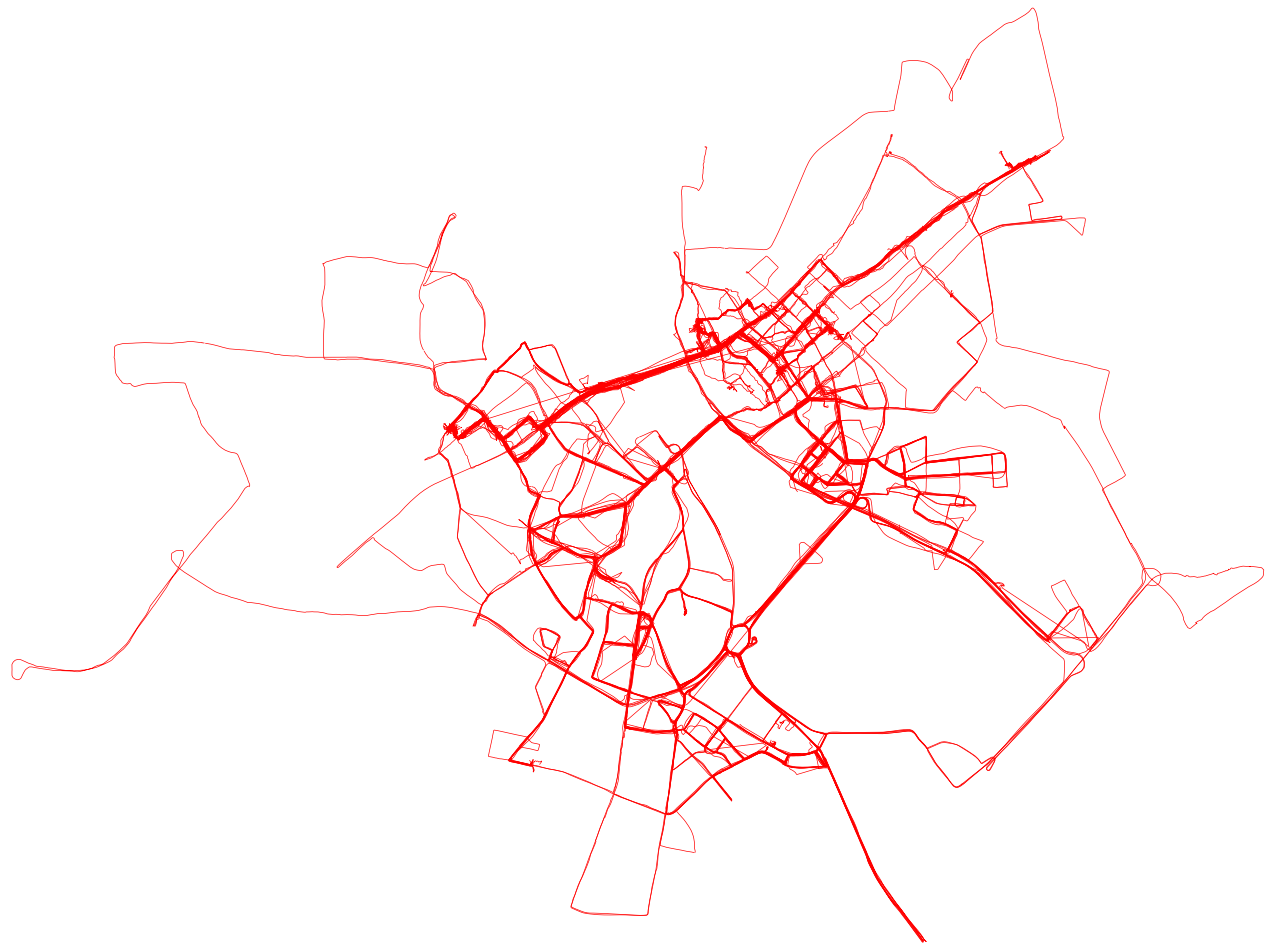
\includegraphics[scale=0.5]{img/all_trails}
  \caption{Ierakstīto datu pārklājums Rīgā}
  \label{fig:all_trails}
\end{figure}

% par(family="AvantGarde")
% k <- kernel("modified.daniell", c(3, 5));
% plot(kernapply(andrejsala$speed[walk], k), type="l", ylim=c(0, 25), xlim=c(0, 900), col="green", lty="dashed", main="Pārvietošanās ātrumi", xlab="Laiks (s)", ylab="Ātrums (m/s)")
% lines(kernapply(andrejsala$speed[drive1], k), type="l", col="red", lty="dotted")
% lines(kernapply(andrejsala$speed[drive2], k), type="l", col="red", lty="dotted")
% lines(kernapply(andrejsala$speed[bike], k), type="l", col="blue", lty="longdash")
% lines(kernapply(homeUni$speed[trolley], k), type="l", col="black", lty="twodash")
% legend(0, 23, c("Iešana", "Auto", "Divritens", "Trolejbuss"), col=c("green", "red", "blue", "black"), lty=c("dashed", "dotted", "longdash", "twodash"))
\section{Pazīmju analīze}
Attēlā \ref{fig:speed_comparison} redzams dažādu transporta līdzekļu pārvietošanās ātrumu grafisks
salīdzinājums. Pārskatāmības labad grafiki nolīdzināti ar \emph{(3, 5)} modificēto Daniell filtru.

Modificētais Daniell filtrs ~\cite{daniell1946} ar platumu $m$ tiek definēts kā 
\begin{eqnarray*}
  w_i = \begin{cases}
    \frac{1}{2 (m - 1)} \text{, ja i = 1 vai i = m}\\
    \frac{1}{m - 1} \text{ citādi}
    \end{cases}
\end{eqnarray*}
Notācija \emph{(3, 5)} nozīmē secīgu filtru ar platumu 3 un 5 pielietošanu, kas ir vienlīdzīga
abu filtru konvolūcijas pielietošanai.

\begin{figure}
  \centering
  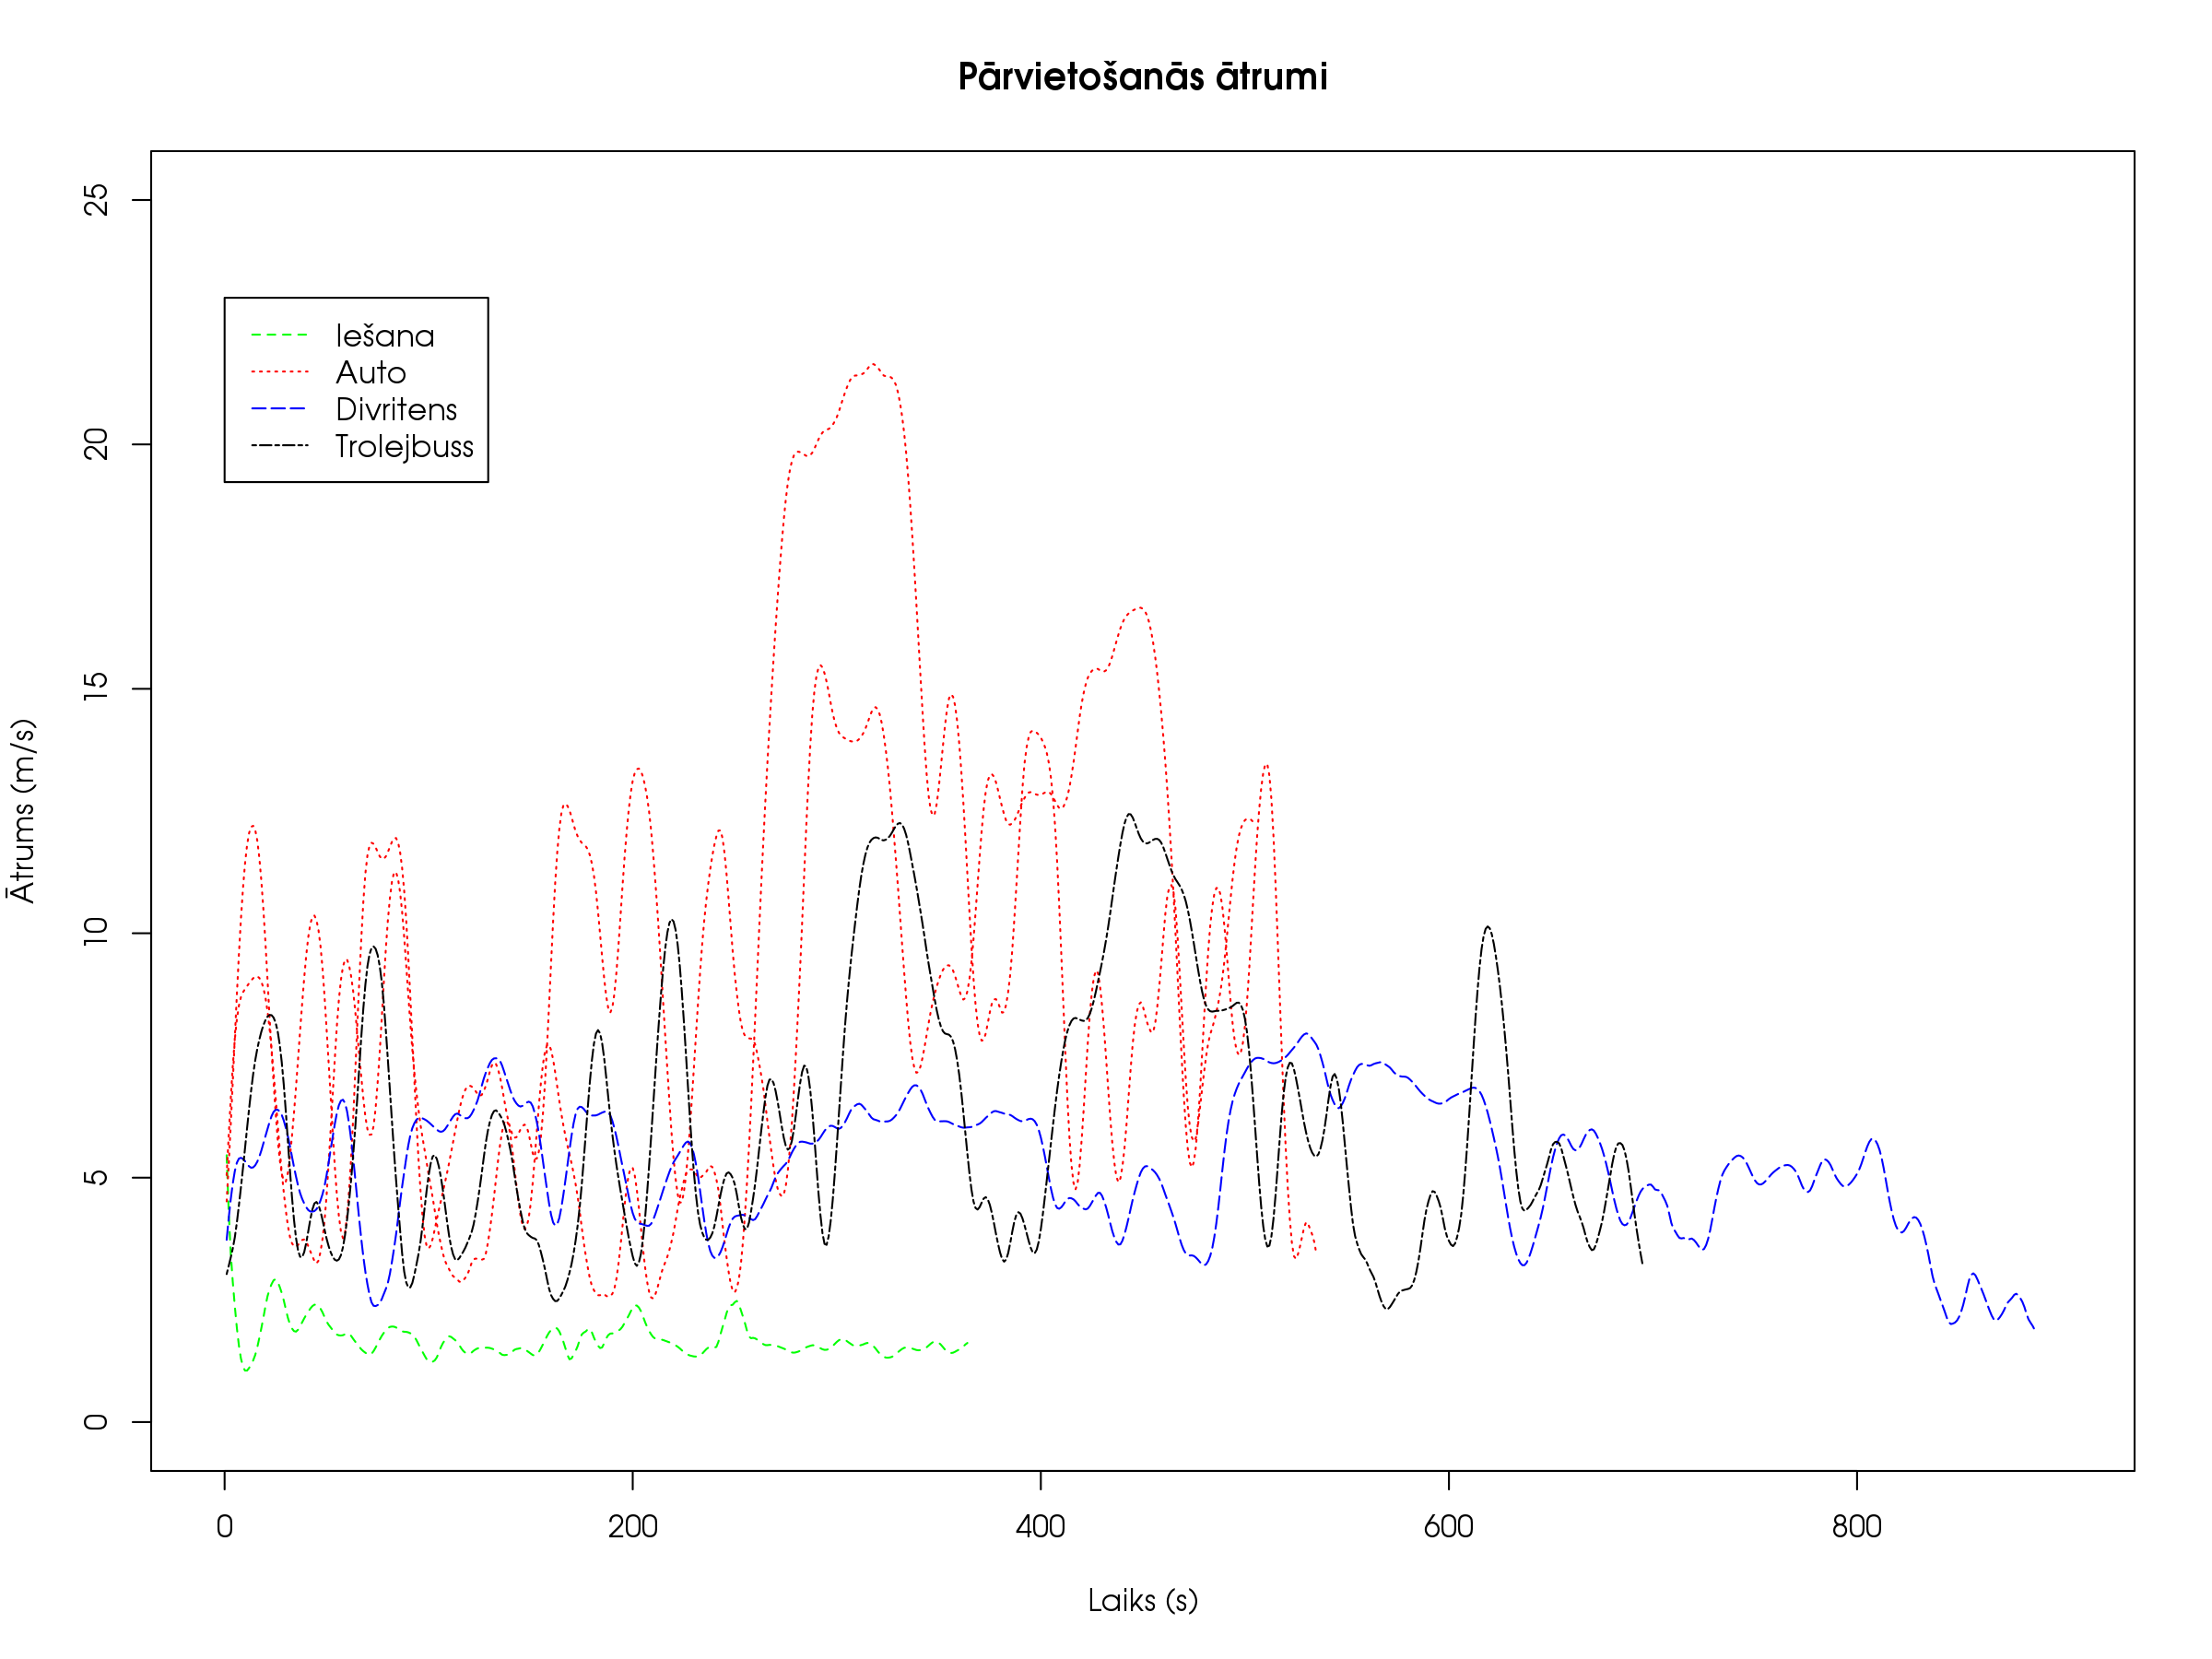
\includegraphics[scale=0.5]{img/speed_comparison}
  \caption{Dažādu transportu pārvietošanās ātrumu salīdzinājums}
  \label{fig:speed_comparison}
\end{figure}

Kā redzams attēlā, dotajā gadījumā cilvēkam ir iespējams salīdzinoši skaidri nošķirt transporta 
veidus jau pēc ātrumiem, taču tikai tad, ja novērojumi veikti pietiekoši ilgā laika periodā.
Attēlā redzams, ka apmēram pirmās 250 - 300 sekundes braukšanu ar trolejbusu, auto un divriteni
ir grūti atšķirt. Zinot lietotos transporta veidus un, galvenokārt, to, ka jāmeklē tieši 4 atšķirīgi,
tos ir iespējams izšķirt, taču šādas zināšanas eksperimenta ietvaros nav dotas.

Attēlā \ref{fig:speed_comparison} redzams arī tas, ka jau tikai pēc ātruma ir viegli nošķirt iešanu
ar kājām no pārējiem pārvietošanās veidiem, kas apstiprina \emph{GeoLife} projekta ietvaros
izstrādāto metodi no sākuma grupēt segmentus grupās ``staigāšana'' un ``ne-staigāšana'' un tikai
pēc tam klasificēt segmentus, kas ir ``ne-staigāšana'' grupā. ~\cite{zheng_gps_segmentation}



% Apzīmējumu Saraksts 6
% 1 Ievads 7
%  1.1 Mērķi 7
%  1.2 Darba struktūra 7
% 2 Bilde no augšas \ Pamatprocesu apraskts 9
%  2.1 Eksistējošie moduļi. 9
%  2.2 Moduļu sadalijums pa izpildāmām programmām 10
% 3 Moduļi 13
%  3.1 Datu iegūšana no pirmkoda 13
%  3.2 Kas ir LEX? 13
%  3.2.1 LEX atslēgvārdi 14
%  3.2.2 LEX\YACC mijiedarbība 18
%  3.3 Pārveidotājs \ “Transformer” 19
%  3.4  Datubāze \ “Primal” 20
%  3.5 Analizētājs \ “Analyser” 20
%  3.6 Organisms \ “Organism” 20
%  3.7 Communicator \ “Communicator” 20
% 4 Datu apstrāde\analīze 21
% 5 Programmas izvada apstrāde 22
% 6 Salīdzinājums ar līdzīgu porgrammatūru 23
% 7 Rezultāti. 24
% 8 Izmantotā literatūra 25
% 9 Pielikumi 26

\literatura{es09260}

\end{document}
